\documentclass[preview]{standalone}

\usepackage{amsmath}
\usepackage{amssymb}
\usepackage{stellar}
\usepackage{definitions}
\usepackage{bettelini}
\usepackage{tikz}

\usetikzlibrary{decorations.markings}

\begin{document}

\id{winding-numbers}
\genpage

\section{Winding number}

\begin{snippetdefinition}{lifting-definition}{Lifting}
    Let \(p \colon \tilde{X} \fromto X\) be a covering
    and \(f \colon Y \fromto X\) a continuous map.
    A \emph{lift} (or \emph{lifting}) of \(f\)
    is a continuous map \(\tilde{f} \colon Y \fromto \tilde{X}\)
    such that \(p \circ \tilde{f} = f\).
\end{snippetdefinition}

\begin{snippettheorem}{path-lifting-theorem}{Path lifting theorem}
    Let \(p \colon \tilde{X} \fromto X\) be a covering,
    \(\alpha \colon [0,1] \fromto X\) a path, and \(\tilde{x}_0 \in p^{-1}(\alpha(0))\).
    Then there exists a unique lift \(\tilde{\alpha} \colon [0,1] \fromto \tilde{X}\)
    with \(\tilde{\alpha}(0) = \tilde{x}_0\).
\end{snippettheorem}

\begin{snippettheorem}{homotopy-lifting-theorem}{Homotopy lifting theorem}
    Let \(p \colon \tilde{X} \fromto X\) be a covering
    and \(F \colon [0,1] \cartesianprod [0,1] \fromto X\) a homotopy.
    If \(\tilde{\alpha}\) is a lift of \(F(\cdot, 0)\)
    starting at \(\tilde{x}_0\), then there exists a unique lift
    \(\tilde{F} \colon [0,1] \cartesianprod [0,1] \fromto \tilde{X}\)
    with \(\tilde{F}(0, 0) = \tilde{x}_0\).
\end{snippettheorem}

\begin{snippetdefinition}{degree-winding-number-definition}{Degree / Winding number}
    Let \(\alpha \colon [0,1] \fromto S^1\) be a loop based at \(1\).
    Let \(\tilde{\alpha}\) be the unique lift with \(\tilde{\alpha}(0) = 0\).
    The \emph{degree} (or \emph{winding number}) of \(\alpha\) is
    \[
        \deg(\alpha) = \tilde{\alpha}(1) \in \integers
    \]
\end{snippetdefinition}

\begin{snippetlemma}{degree-well-defined}{Degree is well-defined on homotopy classes}
    If \(\alpha \simeq \beta\) (rel endpoints), then \(\deg(\alpha) = \deg(\beta)\).
\end{snippetlemma}

\begin{snippetproof}{degree-well-defined-proof}{degree-well-defined}{Degree is well-defined}
    Let \(F\) be a homotopy from \(\alpha\) to \(\beta\) with fixed endpoints.
    By the homotopy lifting theorem, there is a lift \(\tilde{F}\)
    with \(\tilde{F}(0, s) = 0\) for all \(s\).
    Since \(e(\tilde{F}(1, s)) = 1\) for all \(s\),
    we have \(\tilde{F}(1, s) \in \integers\).
    By continuity and connectedness, \(\tilde{F}(1, s)\) is constant.
    Thus \(\tilde{\alpha}(1) = \tilde{F}(1, 0) = \tilde{F}(1, 1) = \tilde{\beta}(1)\).
\end{snippetproof}

\section{Planar curves}

\begin{snippetexample}{winding-numbers-planar-curves-example1}{Winding numbers for planar curves}
    \begin{center}
        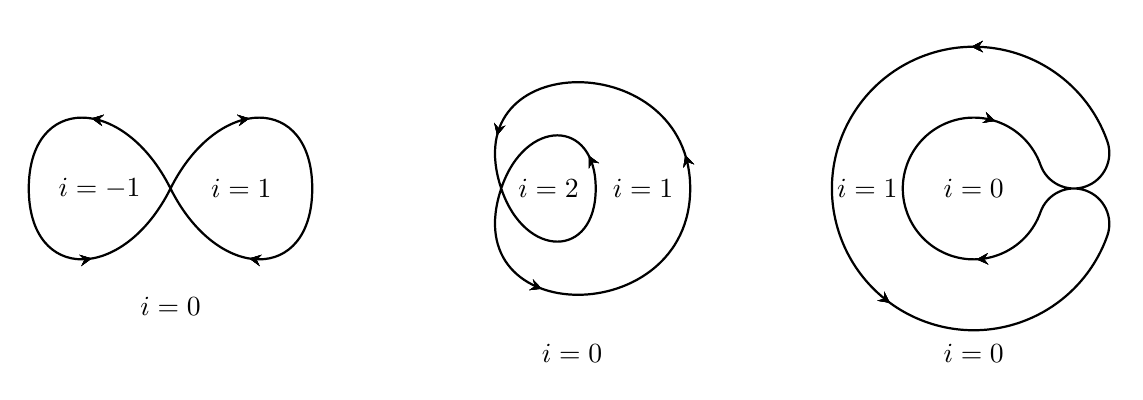
\begin{tikzpicture}[
            scale=0.6,
            >=stealth,
            ->-/.style={decoration={markings, mark=at position #1 with {\arrow{>}}},postaction={decorate}}
        ]
            \draw[thick, ->-=.125, ->-=.375, ->-=.625, ->-=.875] 
                (0,0) .. controls (1,2) and (3,2) .. (3,0) .. controls (3,-2) and (1,-2) .. (0,0) 
                .. controls (-1,2) and (-3,2) .. (-3,0) .. controls (-3,-2) and (-1,-2) .. (0,0);
            \node at (1.5,0) {$i=1$};
            \node at (-1.5,0) {$i=-1$};
            \node at (0,-2.5) {$i=0$};

            \draw[thick, ->-=.125, ->-=.375, ->-=.625, ->-=.875] 
                (7,0) .. controls (6,-3) and (11,-3) .. (11,0) .. controls (11,3) and (6,3) .. (7,0) 
                .. controls (7.5,-1.5) and (9,-1.5) .. (9,0) .. controls (9,1.5) and (7.5,1.5) .. (7,0);
            \node at (8,0) {$i=2$};
            \node at (10,0) {$i=1$};
            \node at (8.5,-3.5) {$i=0$};

            \draw[thick, ->-=.125, ->-=.375, ->-=.7, ->-=.875] 
                ([shift={(17,0)}]19.47:3) 
                arc[start angle=19.47, end angle=340.53, radius=3]
                arc[start angle=-19.47, end angle=160.53, radius=0.75]
                arc[start angle=340.53, end angle=19.47, radius=1.5]
                arc[start angle=199.47, end angle=379.47, radius=0.75];
                
            \node at (14.75,0) {$i=1$};   
            \node at (17,0) {$i=0$}; 
            \node at (17,-3.5) {$i=0$};
        \end{tikzpicture}
    \end{center}
\end{snippetexample}

\end{document}